% --- Sección: Muestreo aproximado de órdenes topológicos ---
\begin{frame}{Sampleo aproximado de órdenes topológicos}
	\dificultyLevel{2}
	En esta sección presentamos un algoritmo probabilístico para \textbf{muestrear órdenes topológicos} de un DAG causal $G$.
	\begin{itemize}[<+- | alert@+>]
		\item A través de este muestreo vamos a poder \textbf{aproximar $ASV$} con precisión creciente según el número de muestras.
		\item La cantidad de muestras necesaria \textbf{crece lentamente} con la precisión deseada.
		\item Nuestro objetivo inicial: \textbf{devolver un orden topológico aleatorio}.
	\end{itemize}
\end{frame}

\begin{frame}{Algoritmo de sampleo}
	\dificultyLevel{3}
		\begin{figure}[ht]
		\centering
		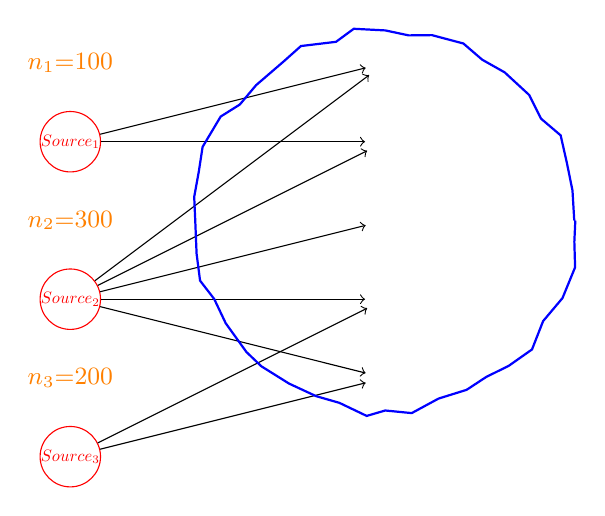
\begin{tikzpicture}
			% Define the right set of nodes
			\foreach \i in {1,2,3,4,5}
			\node[draw=none, circle, minimum size=5mm, inner sep=0pt] (L\i) at (4, -\i) {};
			
			% Define the left set of nodes
			\foreach \j in {1,2,3}
			\node[draw, circle, red, minimum size=5mm, inner sep=0pt] (source\j) at (0, -\j*2) {\scalebox{0.6}{$Source_\j$}};
			
			% Draw edges between nodes (example edges)
			\foreach \i in {1,2}
			\foreach \j in {1,2}
			\draw[->]  (source\j) -- (L\i); 
			
			\foreach \i in {4,5}
			\foreach \j in {2,3}
			\draw[->]  (source\j) -- (L\i); 
			
			\draw[->]  (source2) -- (L3);
			
			\draw [decorate, blue, decoration={random steps, segment length=10pt, amplitude=2pt}, thick]
			(4,-3) circle (2.4);
			
			%Number of órdenes topológicos for each node
			
			\node[draw=none,minimum size=3mm, inner sep=0pt] () at (0, -1) {\small \textcolor{orange}{$n_1$=100}};
			
			\node[draw=none,minimum size=3mm, inner sep=0pt] () at (0, -3) {\small \textcolor{orange}{$n_2$=300}};
			
			\node[draw=none,minimum size=3mm, inner sep=0pt] () at (0, -5) {\small \textcolor{orange}{$n_3$=200}};
		\end{tikzpicture}
		%\caption{Posible comienzo del algoritmo de sampleo, con los candidatos a ser el primer nodo del orden en rojo y el resto del grafo en azul. Cada node fuente (source) tiene sus respectivas cantidades de órdenes topológicos en los que está primero.}
		\label{fig:topoSortSamplingExample}
	\end{figure}
	\pause
	$p(source_1)=\frac{1}{6}, p(source_2)=\frac{1}{2}, p(source_2)=\frac{1}{3}$
\end{frame}

\begin{comment}
	Ejemplo de polytree:
	Los descendientes en común y disjuntos de cada raíz están marcados de un color distinto. Acá hay intersección entre los descendientes por lo que no se los puede mezclar libremente. Por eso tenemos que encontrar otro orden para recorrer el grafo. 
	Conteo de órdenes:
	DFS (sobre el grafo subyacente) enraizado en \(r_i\): los nodos grises ya fueron visitados; los azules está en proceso y los blancos no fueron procesados todavía.
	Calculamos recursivamente para cada componente conexa (del grafo subyacente) no visitada cuáles son sus órdenes topológicos. Necesitamos saber posicion del nodo, tamaño del subárbol y órdenes totales para combinar estos resultados. 
	Luego combinamos los resultados utilizando una función muy similar a la utilizada en el algoritmo recursivo de las clases en la cuál fusionamos ancestros y unrelated. 
	Mencionar que procesamos a los padres e hijos a la vez, por lo que a la hora de fusionarlos tenemos que tener en cuenta esto, lo cuál no es tan sencillo. 
	
	\begin{frame}{Expandiendo el conteo de órdenes}
		\dificultyLevel{2}
		\begin{figure}[ht]
			\centering 
			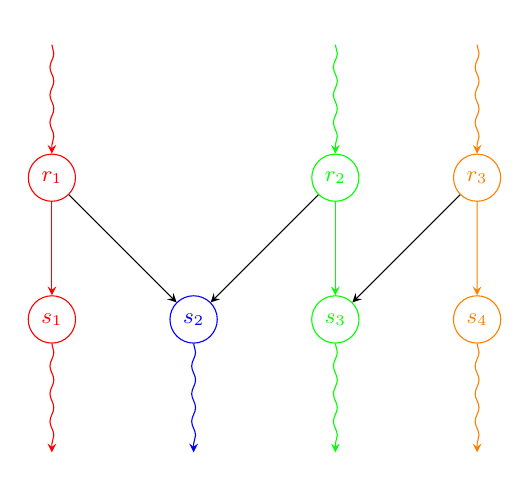
\begin{tikzpicture}[scale=.9, transform shape]
				
				% ---- NODOS ----
				\node[nodo, red] (r1) at (-2,0) {$r_1$};
				\node[nodo, green] (r2) at  (2,0) {$r_2$};
				\node[nodo, orange] (r3) at  (4,0) {$r_3$};
				
				\node[nodo, red] (s1) at (-2,-2) {$s_1$};
				\node[nodo, blue] (s2) at (0,-2) {$s_2$};
				\node[nodo, green] (s3) at (2,-2) {$s_3$};
				\node[nodo, orange] (s4) at (4,-2) {$s_4$};
				
				
				\node[draw=none, fill=none] (h1) at (-2, -4) {};
				\node[draw=none, fill=none] (h1Parent) at (-2, 2) {};
				\node[draw=none, fill=none] (h2) at (0, -4) {};
				\node[draw=none, fill=none] (h3) at (2, -4) {};
				\node[draw=none, fill=none] (h3Parent) at (2, 2) {};
				\node[draw=none, fill=none] (h4) at (4, -4) {};
				\node[draw=none, fill=none] (h4Parent) at (4, 2) {};
				
				
				\path [->] (r1) edge[arista, red]  (s1);
				\path [->] (r1) edge[arista]  (s2);
				\path [->] (r2) edge[arista]  (s2);
				\path [->] (r2) edge[arista, green]  (s3);
				\path [->] (r3) edge[arista]  (s3);
				\path [->] (r3) edge[arista, orange]  (s4);
				
				\path [->] (s1) edge[arista, red, mySnake] (h1);
				\path [->] (h1Parent) edge[arista, red, mySnake] (r1);
				\path [->] (s2) edge[arista, blue,  mySnake]  (h2);
				\path [->] (s3) edge[arista, green,  mySnake]  (h3);
				\path [->] (h3Parent) edge[arista, green,  mySnake]  (r2);
				\path [->] (s4) edge[arista, orange,  mySnake]  (h4);
				\path [->] (h4Parent) edge[arista, orange,  mySnake]  (r3);
				
			\end{tikzpicture}
			\caption{Polytree para el cual no funciona el algoritmo original de conteo.}
			\label{fig:polytreeMultipleIntersections}
		\end{figure}
	\end{frame}
	
	\begin{frame}{Algoritmo de Conteo}
		\dificultyLevel{3}
		\begin{figure}
			\centering
			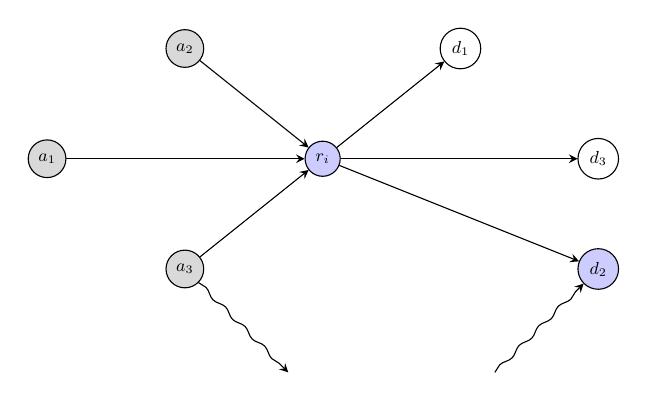
\begin{tikzpicture}[scale=.7, transform shape]
				
				% ---- ESTILOS ----
				\tikzstyle{nodo}      =[circle, draw, minimum size=18pt, font=\small] % estilo base
				\tikzstyle{visited}   =[nodo, fill=gray!30]   % ya visitado
				\tikzstyle{visiting}  =[nodo, fill=blue!20]   % en visita
				\tikzstyle{arista}    =[->, >=stealth]        % aristas
				\tikzstyle{mySnake}   =[decorate, decoration={snake, amplitude=0.7pt}] % para líneas onduladas
				
				% ---- NODOS ----
				\node[visited]  (a1)  at (0,   0) {$a_1$};
				\node[visited]  (a2)  at (2.5,  2) {$a_2$};
				\node[visited]     (a3)  at (2.5, -2) {$a_3$};
				\node[visiting] (xi)  at (5,   0) {$r_i$};
				\node[nodo]  (d_1) at (7.5, 2) {$d_1$};
				\node[visiting]     (d_2) at (10, -2) {$d_2$};
				\node[nodo]     (d_3) at (10,  0) {$d_3$};
				
				% nodos “fantasma” para las líneas onduladas
				\node[draw=none, fill=none] (hijo_a3) at (4.5, -4) {};
				\node[draw=none, fill=none] (hijo_d2) at (8,   -4) {};
				
				% ---- ARISTAS ----
				\path (a1) edge[arista] (xi);
				\path (a2) edge[arista] (xi);
				\path (a3) edge[arista] (xi);
				
				\path (xi) edge[arista] (d_1);
				\path (xi) edge[arista] (d_2);
				\path (xi) edge[arista] (d_3);
				
				\path (a3)      edge[arista, mySnake] node[above right] {} (hijo_a3);
				\path (hijo_d2) edge[arista, mySnake] node[below right] {} (d_2);
			\end{tikzpicture}
			\caption{DFS sobre el grafo subyaciente enraizado en \(r_i\)}
		\end{figure}
	\end{frame}
\end{comment}